	\section{research}
    We propose to build a tool which will visualize the spatiotemporal values of the dataset, visuliaze the output of Machine Learning model and also visualize the points where the mismatches of testing and machine data occur based on the results of the Machine Learning model. We will be using Multi Label Classification Machine Learning Algorithms like support vector machines and existing neural networks to classify the audio files into various categorical sounds. Based on the results of ML model, we will dwell into understanding the mismatches which occur between the annotated and machine predicted data and analyze the causes behind it. 
    
    	\begin{figure}[h!]
    	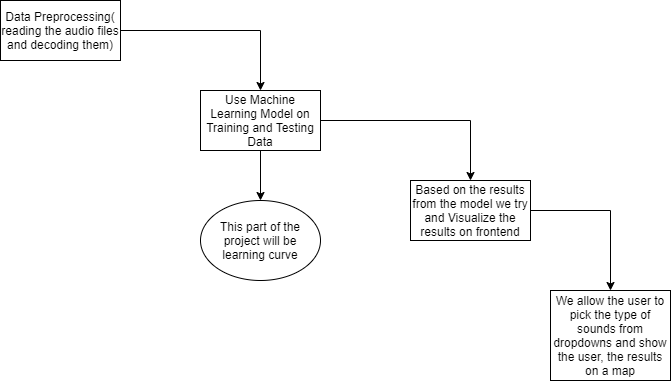
\includegraphics[width=9cm]{figure2}
    	\caption{ Work flow diagram}
    \end{figure}
    
   
   	We have divided the process of building this tool into four stages(see Fig 3) namely data preprocessing state where we process the audio files, Modeling stage where we apply the classification models on the dataset and create REST API's to interact with the front-end, Visualization stage where we visualize the results of machine learning model on the front-end, component building stage where we build components which allows the user to pick spatial and temporal values of various sound samples and display the results on a map.
   	
    This tool would be useful to authorities who monitor sounds around the city which will allow them to pinpoint the location of sound origin.
    
    Initially we started by collecting the dataset for this module which is ~\cite{7}. This is a multi label classification dataset from the urban acoustic sensor network in the city of New York. The next step is to extract the embeddings from the audio data which is collected from 60 different sensors across the city of New York.To do this we implemented an algorithm called Open L3 which is a competitive and deep audio embedding based on the supervised L3-Net.OpenL3 is an improved version of L3-Net, and outperforms VGGish and SoundNet (and the original L3-Net) on several sound recognition tasks.
    
    Next we used a MLP (Multi Layer Perceptron) using a single output layer of size 128 with ReLU activation function and using AutoPool to perfom some pooling functions. We trained the model using SGD (stochastic gradient descent) to reduce binary cross entropy loss. We also used L2-regularization to reduce the weights by adding a penalty term to the loss function.
    
    SGD(stochastic gradient descent) is an iterative method for optimizing an objective function to best fit the model between the actual and predicted output.The main here is to move opposite to the gradient function and update the parameters until we reach the global minima. The learning rate determines the size of steps we take to reach the global minima. We used a learning rate of 0.001 and then with 0.1, we later used an adaptive learning rate optimizer like RMSProp optimizer.
    L2 regularization can deal with multicollinearity problems by constricting the weights in the function. It basically deals with adding L2 penalty which is square of the magnitude of coefficients.
    
    Initially we trained the model on fine level class labels and generated the predictions. Similarly we trained the model on course level labels and generated the corresponding predictions. 
    
    We followed certain metrics to evaluate the performance of our model. The AUPRC (area under precision recall curve ). The AUC curve is plotted with precision against recall with precision on y-axis and recall on x-axis. The area under the AUC curve basically explains the performance of the model against positive examples. This is relative to the number of positive examples in the problem.
    	\begin{figure}[h!]
    	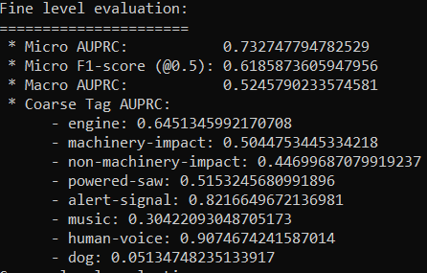
\includegraphics[width=9cm]{figure3}
    	\caption{fine level predictions}
    \end{figure}
   
    
    As we can see from (Fig.4) the model has misclassified certain fine level tags leading to a lower AUPRC of 0.73 on fine level predictions as compared to 0.83 on course levcel predictions.The F1 score recorded for the fine level predictions is 0.61 and 0.73 for course level predictions. As we can observe here the model clearly performed poorly on fine level predictions. This is due to the dense heirarchy of class labels and the model failed to capture all the variance in the data.
    
    We wanted to understand the mismatches caused by the model in these fine-level classes. We performed certain analysis on the predictions by this model on test and validation data. We started with combining the predictions and ground truth for each audio file by using pandas. This made it easy to perform various tests and analysis on our data.
    
   

	
	
